\scanpage{40}
\mspage{\handwritten{8}}
% archive sheet number: 39
is defined as in (7.2 (vii)). We can define, by the same formulas as in (7.2 (vii)and 7.1 (ii)), the morphisms $\handwritten{\unsure{\gamma|\upsilon}}':A'\handwritten{\times}_{S'}B'\handwritten{\longrightarrow}G'$ and $\handwritten{\unsure{\gamma|\upsilon}}'^n:(A'\handwritten{\times}_{S'}B')^n\handwritten{\longrightarrow}G'$, we do have $\handwritten{\unsure{\gamma|\upsilon}}'^n_{(\handwritten{\kappa}(\handwritten{\eta}))}=\handwritten{\unsure{\gamma|\upsilon}}^n_{\handwritten{\eta}}$. Consequently (EGA IV 8.8.3 and 8.10.5\deleted{)}\inserted{and 11.2.6)}\handwritten{,} one can choose $S'$ such that the morphism $\handwritten{\unsure{\gamma|\upsilon}}'^n$\inserted{is flat \handwritten{and}} factors through $D'$, and such that the morphism $(A'\handwritten{\times}_{S'}B')^n\handwritten{\longrightarrow}D'$ deduced from $\handwritten{\unsure{\gamma|\upsilon}}'^n$ is surjective. Then (7.5) the morphism $(A'\handwritten{\times}_{S'}B')^{n+1}\handwritten{\longrightarrow}D'$ deduced from $\handwritten{\unsure{\gamma|\upsilon}}'^{n+1}$ is covering for the fppf topology (and a fortiori for the fpqc topology). Thus $D'$ represents the sheaf associated,for the fppf or fpqc topology, to the presheaf of commutators of $A$ and $B$ in $G$. Moreover, for every $s\handwritten{\in}S'$, the morphism $(A_s\handwritten{\times}_{\handwritten{\kappa}(s)}B_s)^n\handwritten{\longrightarrow}D'_s$ deduced from $\handwritten{\unsure{\gamma|\upsilon}}^n_s$ is surjective; thus (7.6), $(A_s,B_s)$ represents the sheaf of commutators of $A_s$ and $B_s$ in $G_s$ (for the fppf or fpqc topology), whence $D'_s=(A_s,B_s)$.

\uline{Corollary 10.1\handwritten{3}.}- \uline{Let $S$ be an integral prescheme with generic point $\handwritten{\eta}$, $G$ an $S$-group of finite presentation, $D$ a sub-$S$-group prescheme of finite presentation of $G$ with smooth fibers and invariant in $G$. Suppose that we have $(D_{\handwritten{\eta}},D_{\handwritten{\eta}})=D_{\handwritten{\eta}}$ (resp. $(G_{\handwritten{\eta}},D_{\handwritten{\eta}})=D_{\handwritten{\eta}}$). There then exists a nonempty open subset $S'$ of $S$ such that for every $s\handwritten{\in}S'$, we have $(D_s,D_s)=D_s$ (resp. $(G_s,D_{\handwritten{\unsure{e|s}}})=D_s$).}

This follows immediately from (10.12) and from (EGA IV 8.8.2.5).

The statements (10.\handwritten{2}) and \deleted{\unsure{6|b}}\inserted{\handwritten{(}}10.\deleted{\unsure{2}}\inserted{\handwritten{3}}) concerning the category of $S$-groups of finite presentation\handwritten{[}extend to the cat\deleted{\unsure{u}}\inserted{e}gory of pairs formed of an $S$-group of finite presentation and an \deleted{prescheme a} $S$-prescheme of finite presentation with group of operators $G$. More precisely :

\figure{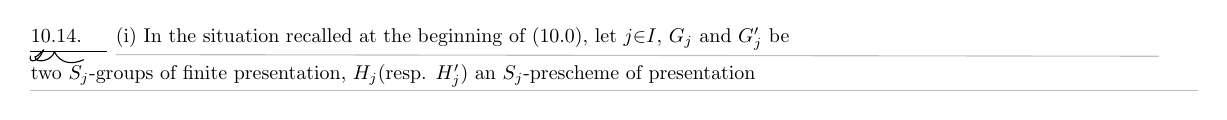
\begin{tikzpicture}[scale=.72,transform shape]
\node[anchor=base west,inner sep=0pt] at (0,0) {10.14.};
\node[anchor=base west,inner sep=0pt] at (1.5,0) {(i) In the situation recalled at the beginning of (10.0), let $j\handwritten{\in}I$, $G_j$ and $G'_j$ be};
\node[anchor=base west,inner sep=0pt] at (0,-.65) {two $S_j$-groups of finite presentation, $H_j$(resp. $H'_j$) an $S_j$-prescheme of presentation};
\handwritten{\draw (0,-.16)--(1.35,-.16);
\draw (0,-.23) .. controls (-.04,-.38) and (.14,-.34) .. (.22,-.15) .. controls (.27,-.06) and (.14,-.25) .. (.08,-.25) .. controls (.08,-.38) and (.39,-.32) .. (.42,-.16) .. controls (.52,-.36) and (.72,-.40) .. (.94,-.30);
\draw[opacity=.25] (1.5,-.21)--(19.9,-.24);
\draw[opacity=.25] (0,-.85)--(20.6,-.85);}
\end{tikzpicture}}
